\documentclass[a4paper,12pt]{report}
\usepackage[italian]{babel}
\usepackage[italian]{cleveref}
\usepackage{fancyhdr, graphicx}

\title{Sistemi Embedded e IoT\\Assignment 03:\\``Smart Garden''}
\author{Davide Merli, Manuel Luzietti, Ryan Perrina}
\date{\today}

\begin{document}

\maketitle
\tableofcontents

\chapter{Struttura generale}

\section{Circuito}
Lo \textit{Smart Garden} si propone di implementare un sistema in grado di monitorare e gestire il comportamento di un giardino. Il circuito, il cui schema è sotto riportato, si compone di:
\begin{itemize}
	\item termistore (sensore di temperatura analogico)
	\item fotoresistore (sensore di luminosità analogico)
	\item 5 led (di cui 4 per l'illuminazione del giardino e uno per verificare lo stato di allarme)
	\item un servomotore per simulare l'irrigazione del giardino
	\item un modulo bluetooth HC-05 (per connessione con l'app)
\end{itemize}

\begin{center}
	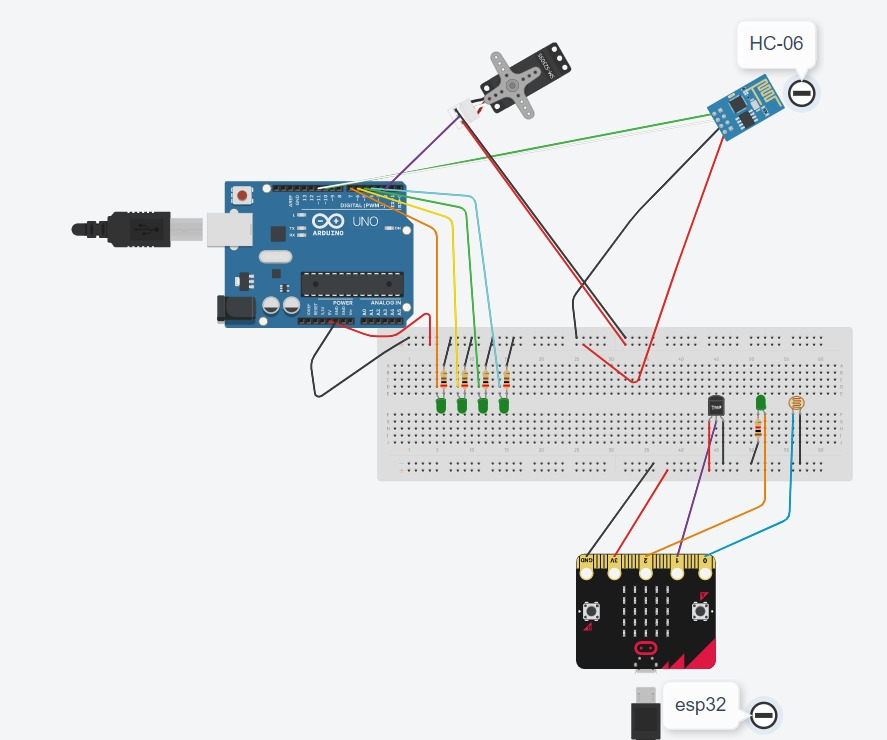
\includegraphics[scale = 0.454]{SchemaCircuito}
	\\figura 1.1: schema del circuito
\end{center}

\section{Architettura}
Lo \textit{Smart Garden} è implementato come una macchina a stati finiti basata su architettura a eventi. Si compone di:
\begin{itemize}
	\item Garden Controller (in esecuzione su Arduino)
	\item Garden Sensorboard (in esecuzione sul modulo ESP-32)
	\item Garden Service (applicazione Java)
	\item Garden Dashboard (pagina web)
	\item Garden App (applicazione Android)
\end{itemize}

\chapter{Descrizione specifica dei componenti}

In questo capitolo verrà descritta la strategia usata per svillupare ciascuna parte.

\section{Garden Controller}
Il \textit{Garden Controller} è la parte dello \textit{Smart Garden} che si occupa di irrigazione e illuminazione. Il sistema ha tre modalità: manuale, automatico e allarme. Le modalità vengono gestite da un macchina a stati finiti asincrona, il cui stato viene modificato da alcuni eventi (es. richiesta del controllo manuale via app). 
\\Il Controller riceve istruzioni dal \textit{Garden Service} (in modalità automatica) o dal {Garden App} (in modalità manuale). Si basa su una coda di eventi, i quali vengono creati al momento della ricezione di messsaggi dalle componenti connesse.

\begin{center}
	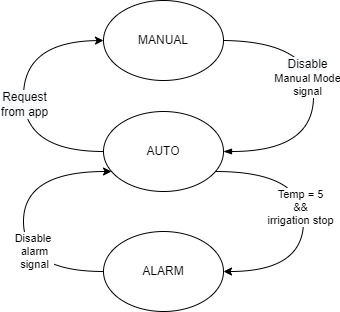
\includegraphics[scale = 0.65]{stateDiagram}
	\\figura 2.1: diagramma degli stati
\end{center}

\section{Garden Sensorboard}
Il \textit{Garden Sensorboard} campiona i dati rilevati dai sensori e li invia attraverso il protocollo MQTT ad un broker online.

\section{Garden Service}
Il \textit{Garden Service} è il cuore dello \textit{Smart Garden} e si occupa di gestire la comunicazione tra le altre componenti.

\section{Garden Dashboard}
La \textit{Garden Dashboard} ha lo scopo di visualizzare su una pagina web i dati ricevuti dal \textit{Garden Service} (stato dei led, luminosità, temperatura e stato della macchina).
\begin{center}
	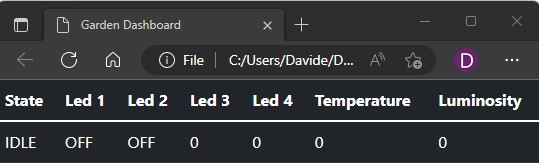
\includegraphics[scale = 0.7]{dashboard}
	\\figura 2.2: Garden Dashboard
\end{center}

\section{Garden App}
La \textit{Garden App} gestisce il comportamento dello \textit{Smart Garden} quando si entra in modalità manuale; inoltre è l'unico in grado di disattivare lo stato di allarme mediante un apposito pulsante.
\begin{center}
	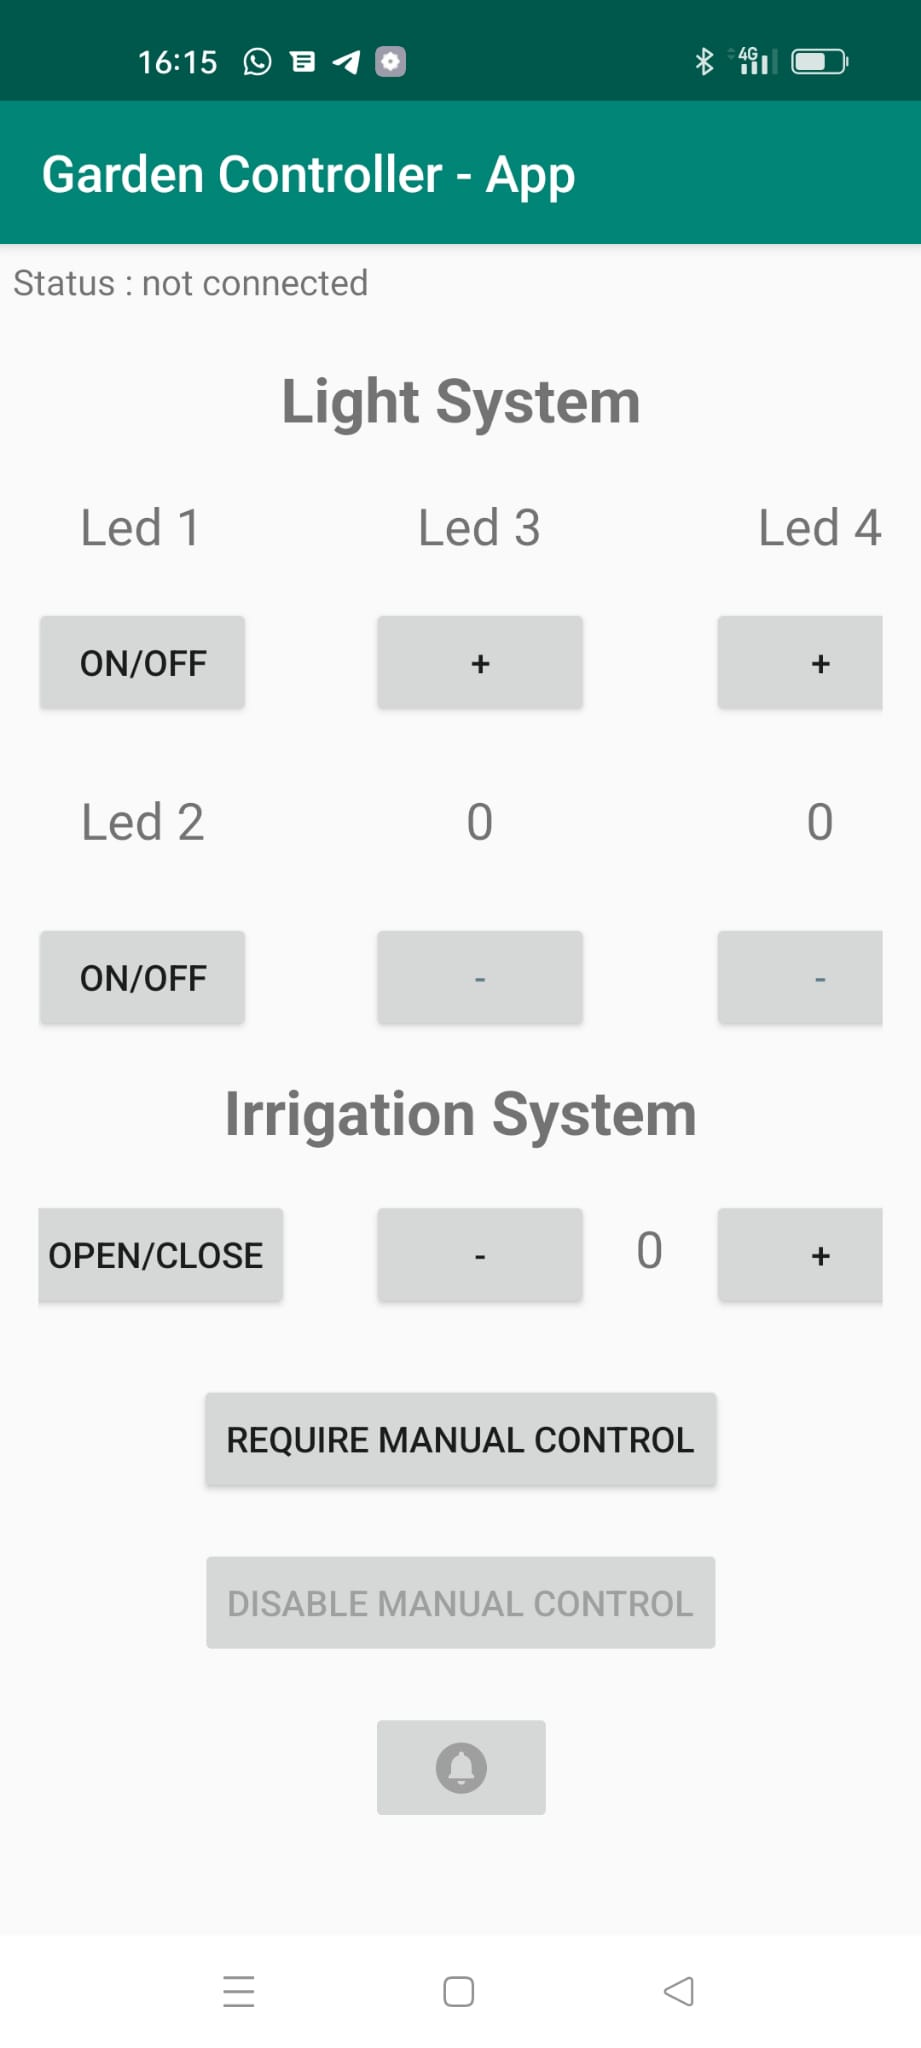
\includegraphics[scale = 0.2]{app}
	\\figura 2.3: Garden App
\end{center}

\end{document}